% chktex-file 2% chktex-file 29
% chktex-file 13
\documentclass{report}
\usepackage{setspace}
\usepackage[a4paper, total={7in, 10in}]{geometry}
\usepackage[fleqn]{amsmath}
\usepackage{empheq}
\usepackage{amssymb}
\usepackage{amsthm}
\usepackage{gensymb}
\usepackage[fleqn]{cases}
\usepackage{multicol}
\usepackage{color}
\usepackage{stix}
\usepackage{chngcntr}
\usepackage{tikz}
\usepackage{enumitem}
\usepackage{pgfplots}
\usepackage{etoolbox}
\usepackage{tikz-3dplot}
\usepackage{tkz-euclide}
\usepackage{graphicx}
\usepackage{enumitem}

\def\nswe#1#2#3{#1\,$#2^\circ\,#3'$}
\graphicspath{ {./assets/} }
\usetikzlibrary{calc,matrix,arrows}
\usetikzlibrary{decorations.pathmorphing,patterns, calligraphy, perspective,backgrounds}

\tikzset{
    right angle quadrant/.code={
            \pgfmathsetmacro\quadranta{{1,1,-1,-1}[#1-1]}     % Arrays for selecting quadrant
            \pgfmathsetmacro\quadrantb{{1,-1,-1,1}[#1-1]}},
    right angle quadrant=1, % Make sure it is set, even if not called explicitly
    right angle length/.code={\def\rightanglelength{#1}},   % Length of symbol
    right angle length=2ex, % Make sure it is set...
    right angle symbol/.style n args={3}{
            insert path={
                    let \p0 = ($(#1)!(#3)!(#2)$) in     % Intersection
                    let \p1 = ($(\p0)!\quadranta*\rightanglelength!(#3)$), % Point on base line
                    \p2 = ($(\p0)!\quadrantb*\rightanglelength!(#2)$) in % Point on perpendicular line
                    let \p3 = ($(\p1)+(\p2)-(\p0)$) in  % Corner point of symbol
                    (\p1) -- (\p3) -- (\p2)
                }
        }
}

\counterwithout{equation}{chapter}
\setlength{\columnseprule}{1pt}
\setlength{\columnsep}{24pt}
\setcounter{chapter}{16}
\hfuzz=100pt

\newcommand{\pgfplotsdrawaxis}{\pgfplots@draw@axis}
\makeatother
\pgfplotsset{only axis on top/.style={axis on top=false, after end axis/.code={
                    \pgfplotsset{axis line style=opaque, ticklabel style=opaque, tick style={thick,opaque},
                        grid=none}\pgfplotsdrawaxis}}}

\newtheorem{theorem}{Theorem}

\begin{document}\makeatletter
\newcommand{\newparallel}{\mathrel{\mathpalette\new@parallel\relax}}
\newcommand{\new@parallel}[2]{%
    \begingroup
    \sbox\z@{$#1T$}% get the height of an uppercase letter
    \resizebox{!}{\ht\z@}{\raisebox{\depth}{$\m@th#1/\mkern-5mu/$}}%
    \endgroup
}
\makeatother

\newcommand{\planelineinter}[5]% a, b, c, p as {a_x,a_y,a_z}, coordinate name
{   \foreach \a [count=\k] in {#1}
        { \ifthenelse{\k=1}{\xdef\tempxa{\a}}
            \ifthenelse{\k=2}{\xdef\tempya{\a}}
            \ifthenelse{\k=3}{\xdef\tempza{\a}}
        }
    \foreach \b [count=\k] in {#2}
        { \ifthenelse{\k=1}{\xdef\tempxb{\b}}
            \ifthenelse{\k=2}{\xdef\tempyb{\b}}
            \ifthenelse{\k=3}{\xdef\tempzb{\b}}
        }
    \foreach \c [count=\k] in {#3}
        { \ifthenelse{\k=1}{\xdef\tempxc{\c}}
            \ifthenelse{\k=2}{\xdef\tempyc{\c}}
            \ifthenelse{\k=3}{\xdef\tempzc{\c}}
        }
    \foreach \p [count=\k] in {#4}
        { \ifthenelse{\k=1}{\xdef\tempxp{\p}}
            \ifthenelse{\k=2}{\xdef\tempyp{\p}}
            \ifthenelse{\k=3}{\xdef\tempzp{\p}}
        }
    \pgfmathsetmacro{\abx}{\tempxb-\tempxa}
    \pgfmathsetmacro{\aby}{\tempyb-\tempya}
    \pgfmathsetmacro{\abz}{\tempzb-\tempza}
    \pgfmathsetmacro{\acx}{\tempxc-\tempxa}
    \pgfmathsetmacro{\acy}{\tempyc-\tempya}
    \pgfmathsetmacro{\acz}{\tempzc-\tempza}
    \pgfmathsetmacro{\nx}{\aby*\acz-\abz*\acy}
    \pgfmathsetmacro{\ny}{\abz*\acx-\abx*\acz}
    \pgfmathsetmacro{\nz}{\abx*\acy-\aby*\acx}
    \pgfmathsetmacro{\d}{(\nx+\ny+\nz)/(\nx*\tempxp+\ny*\tempyp+\nz*\tempzp)}
    \path (0,0,0) -- (#4) coordinate[pos=\d] (#5);
}

% golden ratio and inverse golden ratio
\pgfmathsetmacro{\gr}{(1+sqrt(5))/2}
\pgfmathsetmacro{\igr}{2/(1+sqrt(5))}

%choose axis angles
\newcommand{\xangle}{0}
\newcommand{\yangle}{90}
\newcommand{\zangle}{225}

%choose axis lengths
\newcommand{\xlength}{1}
\newcommand{\ylength}{1}
\newcommand{\zlength}{0.5}

\pgfmathsetmacro{\xx}{\xlength*cos(\xangle)}
\pgfmathsetmacro{\xy}{\xlength*sin(\xangle)}
\pgfmathsetmacro{\yx}{\ylength*cos(\yangle)}
\pgfmathsetmacro{\yy}{\ylength*sin(\yangle)}
\pgfmathsetmacro{\zx}{\zlength*cos(\zangle)}
\pgfmathsetmacro{\zy}{\zlength*sin(\zangle)}

\newcommand{\sol}[1]{

    \noindent \textbf{Sol.}
}
\newcommand{\prooff}[1]{

    \noindent \textbf{Proof.}
}
\newcommand\m[1]{\begin{pmatrix}#1\end{pmatrix}}
\newcommand\vm[1]{\begin{vmatrix}#1\end{vmatrix}}
\newenvironment{amatrix}[1]{%
    \left(\begin{array}{@{}*{#1}{c}|c@{}}
        }{%
    \end{array}\right)
}
\newenvironment{cequation}{
    \makeatletter
    \setbool{@fleqn}{false}
    \makeatother
    \begin{equation*}
        }{\end{equation*}}

\begin{titlepage}
    \raggedleft{}
    \rule{1pt}{\textheight}
    \hspace{0.02\textwidth}
    \parbox[b]{0.75\textwidth}{

    {\Huge\bfseries Solution Book of \\[0.5\baselineskip] Mathematic}\\[2\baselineskip]
    {\large\textit{Ssnior 2 Part I}}\\[4\baselineskip]
    {\Large\textsc{MELVIN CHIA}}

    \vspace{0.5\textheight}

    {\noindent Written on 9 October 2022}\\[\baselineskip]
    }

\end{titlepage}

\doublespacing{}
\tableofcontents
\singlespacing{}
\newpage

\begin{multicols}{2}

    \section{Longitude and Latitude}

    The earth is approximately spherical in shape, its radius is about $6,370km$,
    and its axis is a line that passes through the north ({$N$}) and south ($S$)
    poles. The earth rotating around its axis once is called a day, and the earth
    rotating around the sun once is called a year.

    Any point on the earth's surface can be identified by two angles, the first is
    the angle between the point and the equator, called the \emph{latitude} of the
    point, and the second is the angle between the point and the prime meridian,
    called the \emph{longitude} of the point.

    \subsection*{Longitude and Lines of Longitude}

    The two semicircles that are formed by the intersection of the earth's surface
    with the plane that passes through the north and south poles are called the
    \emph{lines of longitude}, also called \emph{meridians}. The lines of longitude
    that passes through the \emph{Greenwich Observatory} in England are considered
    as $0^{\circ}$ longitude, called the \emph{Greenwich Meridian} or \emph{prime
        meridian}.

    \begin{center}
        \includegraphics[scale=0.25]{primemeridian}
    \end{center}

    The angle between the Greenwich Meridian and the line of longitude that passes
    through the point $P$ is called the \emph{longitude of $P$}. There are 360
    degrees of longitude ($+180^\circ$ eastward and $-180^\circ$ westward.). The
    prime meridian divides the world into the Eastern Hemisphere and the Western
    Hemisphere. $180^{\circ}E$ and $180^{\circ}W$ coincide with each other at the
    same line of longitude, called the \emph{$180^{th}$ Meridian} or
    \emph{Antimeridian}.

    \begin{center}
        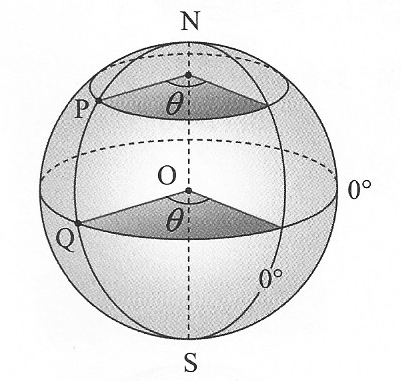
\includegraphics[scale=1.4]{longitude.png}
    \end{center}

    \subsection*{Latitude and Parallels of Latitude}

    The lines of latitude are the circles that are perpendicular to the plane that
    passes through the north and south poles. The \emph{equator} is the one and
    only great circle among the parallels of latitude.

    \begin{center}
        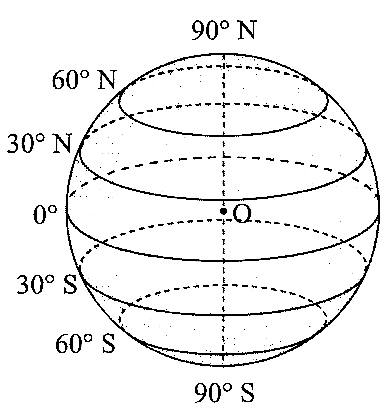
\includegraphics[scale=1.3]{latitude}
    \end{center}

    The angle between the equator and the line of latitude that passes through the
    point $P$ is called the \emph{latitude of $P$}. There are 180 degrees of
    latitude ($+90^\circ$ northward and $-90^\circ$ southward). The equator divides
    the world into the Northern Hemisphere and the Southern Hemisphere.

    \begin{center}
        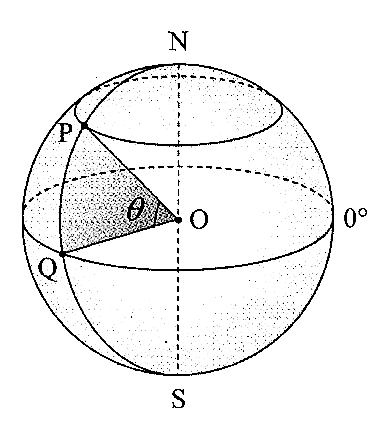
\includegraphics[scale=1.3]{latitude 2.png}
    \end{center}

    \subsection{Practice 3}

    \begin{enumerate}
        \item In the diagram below, $NGS$ is the prime meridian, $O$ is the centre of the
              earth. Find the longitude of locations $P$, $Q$, $R$ and $T$.
              \begin{center}
                  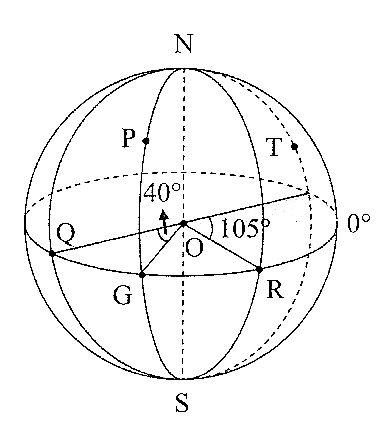
\includegraphics[scale=1.3]{p3q1.png}
              \end{center}
        \item In the diagram below, $O$ is the centre of the earth, location $A$ and $B$ are
              on the equator. Find the location of $P$, $Q$, $R$ and $T$.
              \begin{center}
                  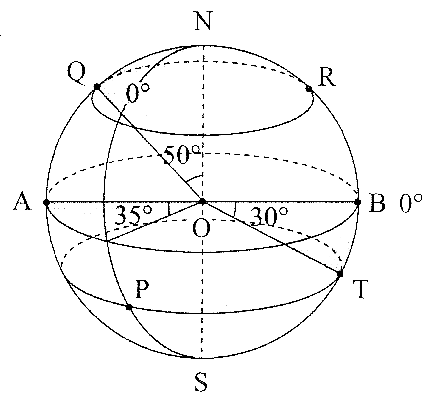
\includegraphics[scale=1.3]{p3q2.png}
              \end{center}
    \end{enumerate}

    \subsection*{Radius of the Parallel of Latitude}

    Let $R$ be the radius of the earth, $r$ be the radius of latitude $\theta$,
    then $r = R \cos \theta$.
    \begin{center}
        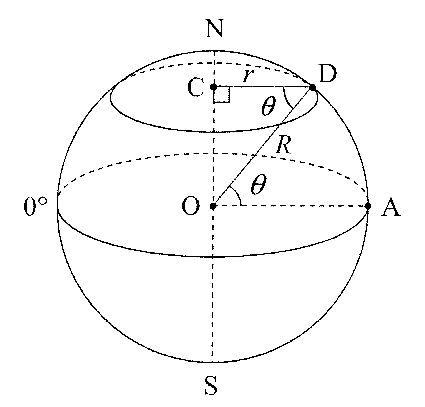
\includegraphics[scale=1.3]{radius of latitude.png}
    \end{center}

    \subsection*{Nautical Miles}

    The arc length corresponding to $1'$ ($=\frac{1}{60}^\circ$) of the great
    circle on earth is called a \emph{nautical mile} ($1$\emph{NM}), that is,
    $1\text{\emph{NM}} = \frac{1}{60 \times 360} \times 2\pi \times 6370km =
        1.853km$.

    \subsection*{Time Difference and Longitude}

    The time is calculated by the rotation of the earth around its axis. The earth
    rotates around its axis from west to east once in $24h$. That is, the earth
    rotates $15^\circ$ in $1h$. Thus, the time difference between two locations on
    the earth is equal to the difference of their longitudes. Thus, the time
    difference is $1hr$ per $15^\circ$ of longitude difference.

    \begin{enumerate}[listparindent=1.5em]
        \item \textbf{Local Time}\\
              The local time is the time at a location on the earth. The local time for any location on the same line of longitude is the same.
        \item \textbf{Standard Time}\\
              Back in the year $1844$, International Meridian Conference was held in Washington DC. The conference decided to divide the world into 24 time zones based on the Greenwich Meridian, called the \emph{Greenwich Meridian Time (GMT)}. There is zero time offset $7.5^\circ$ eastward and $7.5^\circ$ westward of the Greenwich Meridian. The time offset is $1hr$ per $15^\circ$ of longitude difference. All places in the same time zone share the same local time with the location located on the line of longitude that passes through the centre of the time zone, called the \emph{standard time} or \emph{zone time}.

              \indent When entering a new time zone from the east, the local time is advanced by
              $1hr$ per $15^\circ$ of longitude difference. When entering a new time zone
              from the west, the local time is delayed by $1hr$ per $15^\circ$ of longitude
              difference.
    \end{enumerate}
\end{multicols}
\begin{center}
    \makebox[\textwidth]{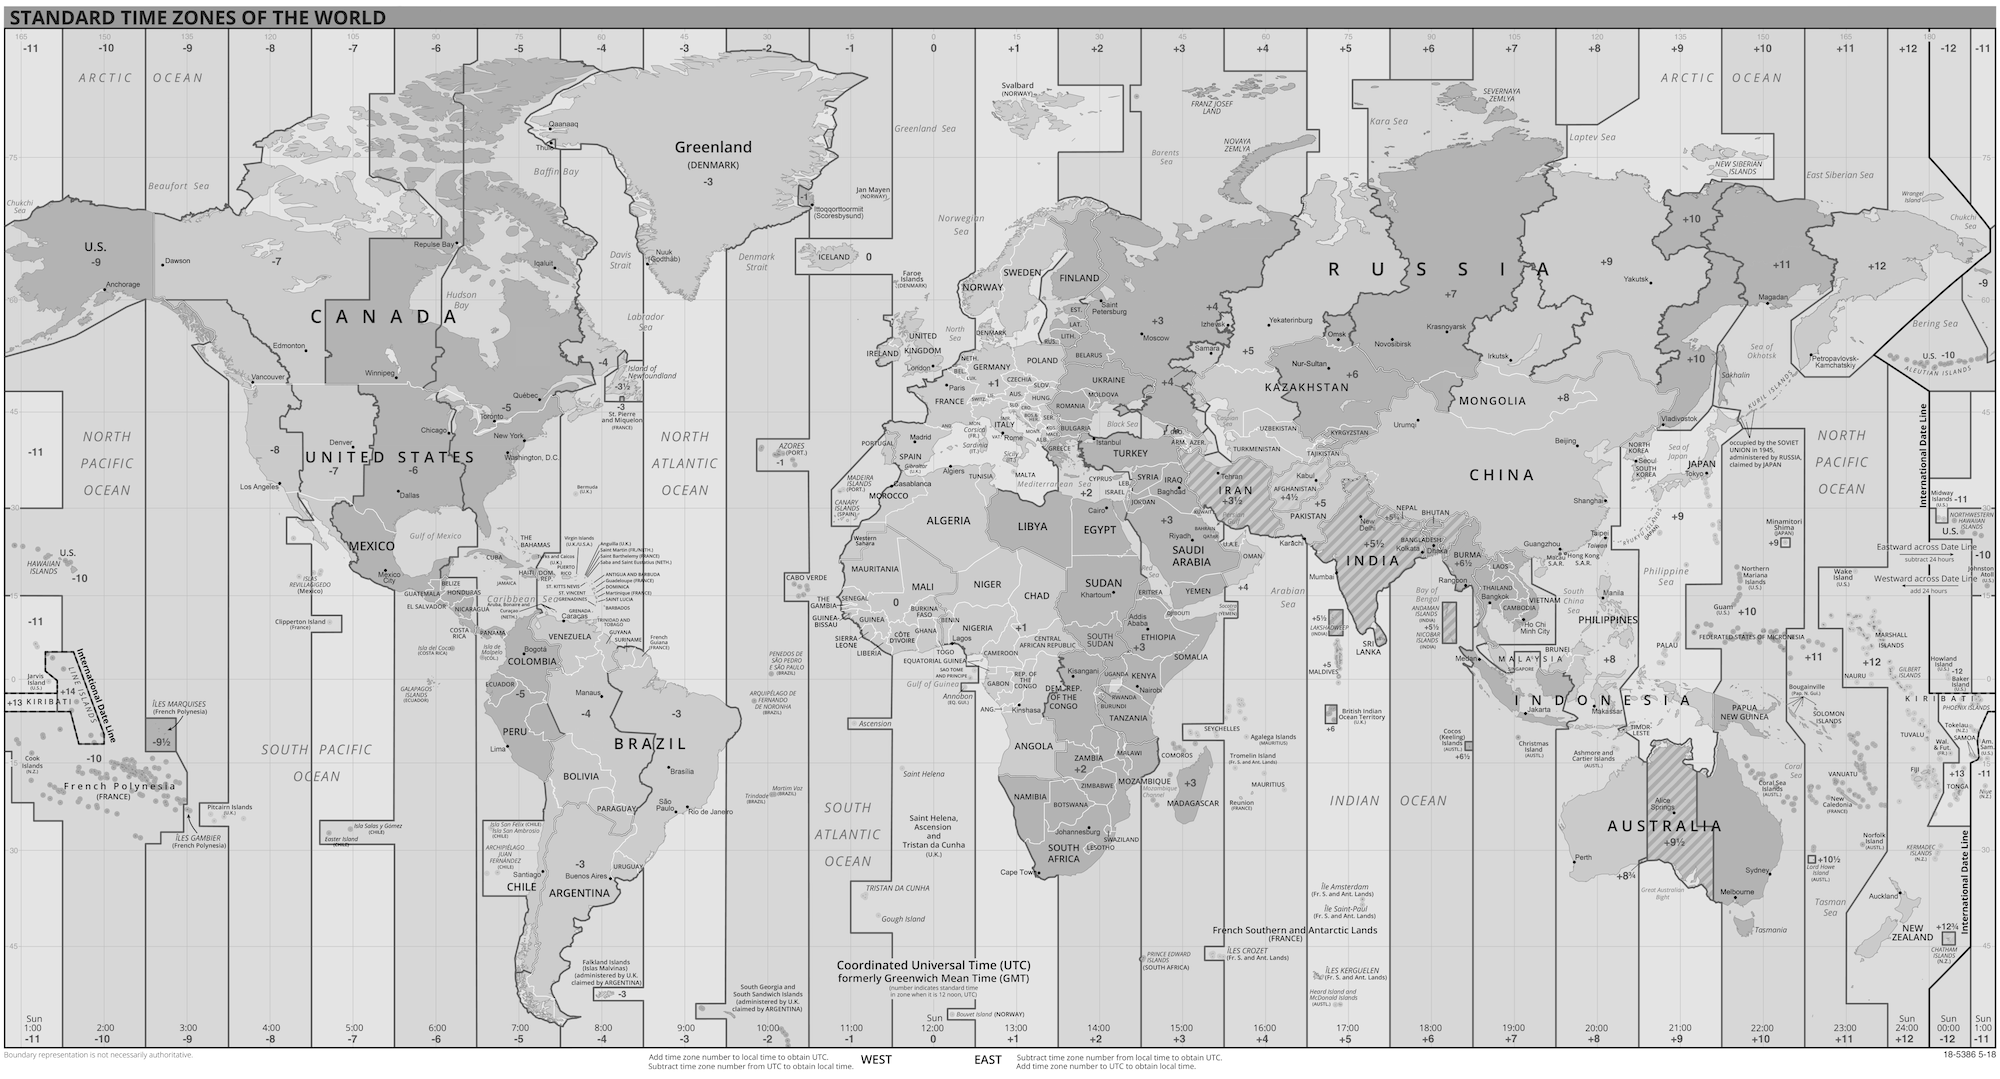
\includegraphics[scale=0.42]{timezone.png}}
\end{center}
\begin{multicols}{2}
    \section{Distance of Two Locations on the Same Line of Longitude}

    The distance of two location on the same line of longitude is the arc length
    corresponding to the difference of their latitudes. Given two location $P$ and
    $Q$ on the same line of longitude, according to the definition of nautical
    mile, the distance between $P$ and $Q$ can be acquired by the arc length of
    $PQ$. That is, $\overset{\frown}{PQ} = \theta \times 60$\emph{NM}, where
    $\theta$ is the difference of their latitudes.

    \begin{center}
        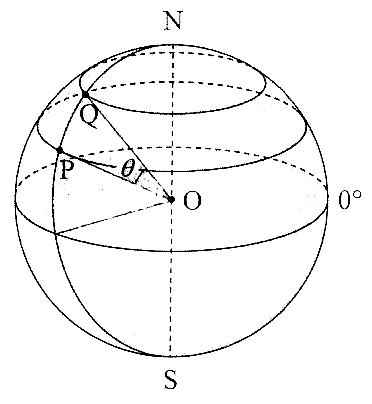
\includegraphics[scale=1.4]{longitude difference.png}
    \end{center}

    \subsection{Practice 4}

    \begin{enumerate}
        \item Given that location $A$ and $B$ are on the same line of longitude. Based on the
              following longitude, find the distance between $A$ and $B$ (Express your answer
              in nautical miles):
              \begin{enumerate}
                  \item $A(50^\circ N)$, $B(75^\circ N)$
                  \item $A(0^\circ)$, $B(42^\circ S)$
                  \item $A(43^\circ N)$, $B(38^\circ S)$
              \end{enumerate}
        \item Given that location $P$ and $Q$ are on the same line of longitude. The distane
              between two locations is $1000$\emph{NM}, $P$ is located at $7^\circ 30'$ north
              of the equator. Based on the following criteria, find the latitude of $Q$:
              \begin{enumerate}
                  \item $Q$ is located at the north of $P$
                  \item $Q$ is located at the south of $P$
              \end{enumerate}
    \end{enumerate}

    \subsection{Exercise 17.5}

    \begin{enumerate}
        \item Given that $A$ and $B$ are on the same line of longitude. Based on the
              following difference of latitude of two locations, find the distance between
              $A$ and $B$ (Express your answer in nautical miles):
              \begin{enumerate}
                  \item $\theta = 39^\circ$
                  \item $\theta = 80^\circ 30'$
                  \item $\theta = 64^\circ 20'$
              \end{enumerate}
        \item Given that $A$ and $B$ are on the same line of longitude. Based on the
              following distance between two locations, find the difference of latitude of
              $A$ and $B$ (Round your answer to the nearest minute):
              \begin{enumerate}
                  \item $700$\emph{NM}
                  \item $318$\emph{NM}
                  \item $3450$\emph{NM}
              \end{enumerate}
        \item Find the distance between two locations along the same line of longitude:
              \begin{enumerate}
                  \item $A(21^\circ S, 110^\circ E)$, $B(33^\circ S, 110^\circ E)$
                  \item $X(38^\circ N, 40^\circ W)$, $Y(19^\circ N, 40^\circ W)$
                  \item $E(34^\circ 45' S, 80^\circ E)$, $F(0^\circ, 80^\circ E)$
                  \item $P(18^\circ 15' N, 90^\circ W)$, $Q(43^\circ 30' N, 90^\circ W)$
                  \item $T(15^\circ 30' N, 120^\circ E)$, $M(24^\circ 30' N, 120^\circ E)$
              \end{enumerate}
        \item Location $X$ and $Y$ are on the same line of longitude, the distane between
              them is $400$\emph{NM}. Find the difference of latitude of $X$ and $Y$.
        \item Location $P$ and $Q$ are on the same line of longitude, and their distance
              along the line of longitude is $600$\emph{NM}, find the difference between
              their latitude.
        \item $X$ city and $Y$ city are on the same line of longitude, the latitude of $X$ city is $2^\circ 15'$ north of the equator, the latitude of $Y$ city is $6^\circ$ north of the equator. Find the distance between $X$ city and $Y$ city (Express your answer in kilometers).
        \item A plane is flying $1000km$ due north from airport $A(15^\circ N, 115^\circ E)$
              to airport $B$. Find the longitude and latitude of airport $B$.
        \item A plane is flying $1500km$ due south from airport $A(5^\circ N, 100^\circ E)$
              to airport $B$. Find the longitude and latitude of airport $B$.
        \item Find the distance from $A(18^\circ 30' S)$ to the north pole along the same
              line of longitude.
        \item The distance between location $C$ and $D$ is $700$\emph{NM}, $C$ is located at
              $5^\circ 30'$ north of the equator. Find the latitude of $D$.
        \item A plane takes off from $P(60^\circ N, 60^\circ E)$ and flies pass north pole
              along the great circle route to $Q(50^\circ N, 120^\circ W)$. Find the flying
              distance.
        \item A ship sails from $P(50^\circ S, 160^\circ E)$ due north to another port
              $Q(30^\circ N, 160^\circ E)$. The sailing time is 10 days. Find the average
              speed of the ship. (Express your answer in \emph{NM}$/hr$)
        \item Given that $PQ$ is the diameter of the parallel of latitude $35^\circ S$. A
              plane takes off from location $P$, flies pass the south pole along the line of
              longitude, and lands at location $Q$ after $13hrs 40mins$. Find the average
              speed of the plane for the whole flight duration. (Express your answer in
              \emph{NM}$/hr$)
    \end{enumerate}

    \section{Distance of Two Locations on the Same Parallel of Latitude}

    The distance between two locations on the same parallel of latitude is the arc
    length on the parallel of latitude corresponding to the difference of their
    longitudes.

    \begin{center}
        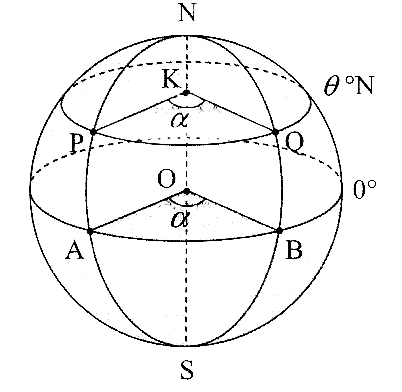
\includegraphics[scale=1.4]{latitude difference.png}
    \end{center}

    In the diagram above, $P$ and $Q$ are on the same parallel of latitude
    $\theta$, their difference of latitude is $\alpha$. $A$ and $B$ are locations
    on the equator.

    Given that $\angle PKQ = \angle AOB = \alpha$. Let $R$ be the radius of the
    earth, $r$ be the radius of the parallel of latitude.

    \begin{flalign*}
        \frac{\overset{\frown}{PQ}}{\overset{\frown}{AB}} & = \frac{\frac{\alpha}{360^\circ} \times 2\pi r}{\frac{\alpha}{360^\circ} \times 2\pi R} \\
                                                          & = \frac{r}{R}                                                                           \\
    \end{flalign*}

    From the radius of the the parallel of latitude $r = R \cos R$, we have
    $\frac{r}{R} = \cos \theta$.
    \begin{flalign*}
        \therefore \frac{\overset{\frown}{PQ}}{\overset{\frown}{AB}} & = \cos \theta                                             \\
        \overset{\frown}{PQ}                                         & = \overset{\frown}{AB} \times \cos \theta                 \\
                                                                     & = \alpha \times 60 \times \cos \theta \text{\emph{NM} or} \\
                                                                     & = \alpha \times 60 \times \cos \theta \times 1.853km
    \end{flalign*}

    \subsection{Practice 5}

    \begin{enumerate}
        \item Fidn the distance of the following pairs of location on the same parallel of
              latitude (Express your answer in nautical miles):
              \begin{enumerate}
                  \item $P(80^\circ N, 105^\circ W), Q(80^\circ N, 48^\circ W)$
                  \item $M(50^\circ S, 48^\circ E), N(50^\circ S, 100^\circ E)$
                  \item $X(40^\circ N, 28^\circ 15' E), Y(40^\circ N, 42^\circ 45' W)$
                  \item $K(20^\circ S, 160^\circ E), L(20^\circ S, 140^\circ W)$
              \end{enumerate}
        \item Given that $A$ is located at the west of $B(46^\circ N, 72^\circ W)$ with a
              distance of $2350$\emph{NM}. Find the longitude and latitude of $A$.
    \end{enumerate}
    \subsection{Exercise 17.6}
    \begin{enumerate}
        \item Find the distance of the following pairs of location on the same parallel of
              latitude (Express your answer in nautical miles):
              \begin{enumerate}
                  \item $P(45^\circ S, 20^\circ E), Q(45^\circ S, 100^\circ E)$
                  \item $M(36^\circ N, 45^\circ W), N(36^\circ N, 105^\circ W)$
                  \item $A(80^\circ S, 130^\circ E), B(80^\circ S, 165^\circ E)$
                  \item $K(70^\circ N, 40^\circ E), L(70^\circ N, 20^\circ W)$
                  \item $T(0^\circ, 128^\circ W), M(0^\circ, 120^\circ E)$
              \end{enumerate}
        \item Based on the following distances of location $P$ and $Q$ and the longitude and
              latitude of $P$, find the longitude and latitude of $Q$:
              \begin{enumerate}
                  \item $PQ = 800$\emph{NM}, $Q$ is located at the west of $P(50^\circ S, 100^\circ W)$
                  \item $PQ = 3400$\emph{NM}, $Q$ is located at the east of $P(35^\circ N, 68^\circ E)$
                  \item $PQ = 1450$\emph{NM}, $Q$ is located at the east of $P(42^\circ N, 150^\circ W)$
              \end{enumerate}
        \item Given that two places are on the parallel of latitude $60^\circ$ north to the
              equator, and their difference of longitude is $160^\circ$. Find the distance of
              the two places. (Express your answer in kilometers)
        \item City $A$ and $B$ are on the parallel of latitude $5^\circ 30'$ north to the
              equator, their longitude are $100^\circ 15' E$ and $103^\circ E$ respectively.
              Find the distance between two cities along the parallel of latitude.
        \item Find the circumference of the parallel of latitude $35^\circ 30' S$.
        \item Find the radius of the parallel of latitude $60' N$.
        \item A ship set sail from $P(20^\circ E)$ and sail $600$\emph{NM} due east along
              $42^\circ N$ parallel of latitude. Find the longitude and latitude of the
              destination.
        \item A ship sails from port $P(48^\circ N, 12^\circ W)$ $1000$\emph{NM} due west to
              another port $Q$, find the longitude and latitude of $Q$.
        \item Given that $A$ is located at the east of Paris$(49^\circ N, 2^\circ 30' E)$
              with a distance of $2200km$. Find the longitude and latitude of $A$.
        \item A plane flies from $X(40^\circ N, 2^\circ 30' E)$ $9265km$ due east to $Y$,
              find the longitude and latitude of $Y$.
        \item Given that the earth takes $24hrs$ to rotate once. Find the speed of Kuala
              Lumpur$(3^\circ 15' N, 102^\circ E)$ to rotate once. (Express your answer in
              \emph{NM}$/hr$)
        \item Given that the longitude of $P$ and $Q$ are $50^\circ$ and $100c^\circ$
              respectively. If $P$ and $Q$ both located at the west of $R(55^\circ S)$ and
              $PR = PQ$, find:
              \begin{enumerate}
                  \item The longitude of $R$.
                  \item Th distance between $Q$ and $R$ along the parallel of latitude.
              \end{enumerate}
        \item A plane flies from $F(50^\circ S, 50^\circ E)$ due west to $H(50^\circ S,
                  45^\circ W)$, then flies from $H$ due north $4800$\emph{NM} to $K$. Given that
              the average speed of the plane is $480\text{\emph{NM}}/hr$ throughout the
              journey, find:
              \begin{enumerate}
                  \item The latitude of $K$.
                  \item The distance between $F$ and $H$ along the parallel of latitude.
                  \item The flight duration for the whole journey.
              \end{enumerate}
    \end{enumerate}

    \section{Revision Exercise 17}

    \begin{enumerate}
        \item In the cuboid shown below, $FG = 10cm$, $GH = 7cm$, $DH = 8.4cm$, find:
              \begin{enumerate}
                  \item The angle formed by angle $AC$ and plane $BFGC$.
                  \item The angle formed by angle $FD$ and plane $EFGH$.
              \end{enumerate}
              \begin{center}
                  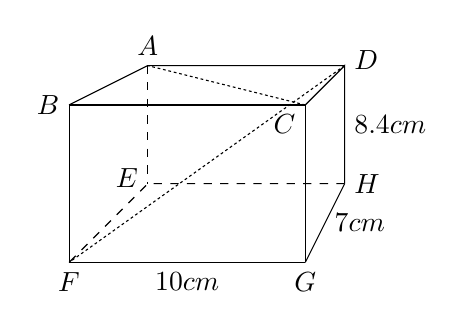
\begin{tikzpicture}
                      \draw (0,0) node [below] {$F$} --(3,0) node [below] {$G$} node[midway, below] {$10cm$};
                      \draw (3,0)--(3.5,1) node [right] {$H$} node [midway, right] {$7cm$};
                      \draw[dashed] (3.5,1)--(1,1) node [above=2pt, left] {$E$} --(0,0);
                      \draw (0,0)--(0,2) node[left] {$B$}--(3,2) node[below left] {$C$} --(3,0);
                      \draw (0,2)--(1,2.5)--(3.5,2.5) node[above=2pt, right] {$D$};
                      \draw (3,2)--(3.5,2.5)--(3.5,1) node [midway, right] {$8.4cm$};
                      \draw[dashed] (1,2.5) node [above] {$A$} --(1,1);
                      \draw[dash pattern=on 1pt off 1pt] (3.5,2.5) -- (0,0);
                      \draw[dash pattern=on 1pt off 1pt] (3,2) -- (1, 2.5);
                  \end{tikzpicture}
              \end{center}
        \item The diagram below shows a cuboid with volume of $400cm^3$, height of $10.5cm$,
              $AD = 2DC$. Find the angle formed by angle $AG$ and plane $ADHE$.
              \begin{center}
                  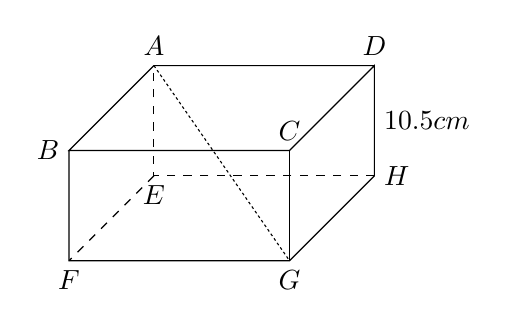
\begin{tikzpicture}[scale=1.4]
                      \draw (2,1,0) node [above] {$D$} --(0,1,0) node [above] {$A$} --(0,1,2) node [left] {$B$} --(2,1,2)node [above] {$C$} --(2,1,0) --(2,0,0) node [right] {$H$} node [midway, right] {$10.5cm$} --(2,0,2) node [below] {$G$} --(0,0,2) node [below] {$F$} --(0,1,2);
                      \draw (2,1,2)--(2,0,2);
                      \draw[dashed](2,0,0)--(0,0,0) node [below] {$E$}--(0,1,0);
                      \draw[dashed](0,0,0)--(0,0,2);
                      \draw[dash pattern=on 1pt off 1pt] (0, 1, 0) -- (2, 0, 2);
                  \end{tikzpicture}
              \end{center}
        \item The diagram below shows a reception room with a square floor with side length
              of $6m$. Given that the elevation angle of corner $C$ measured from corner $A$
              is $30^\circ$, find the angle formed by the line connecting corner $A$ and $B$
              with the floor.
              \begin{center}
                  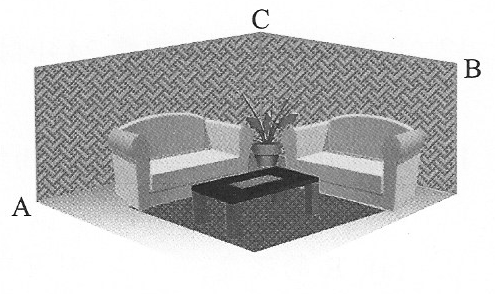
\includegraphics{reception.png}
              \end{center}
        \item The diagram below shows a cuboid with length of $8cm$, width of $5cm$ and
              height of $6cm$, $M$ is the midpoint of $BF$. Find the angle formed by plane
              $HDM$ and plane $ADHE$.
              \begin{center}
                  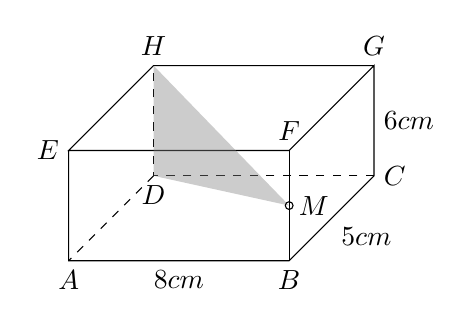
\begin{tikzpicture}[scale=1.4]
                      \draw (2,1,0) node [above] {$G$} --(0,1,0) node [above] {$H$} --(0,1,2) node [left] {$E$} --(2,1,2)node [above] {$F$} --(2,1,0) --(2,0,0) node [right] {$C$} node [midway, right] {$6cm$} --(2,0,2) node [below] {$B$}  node [midway, below right] {$5cm$} --(0,0,2) node [below] {$A$}  node [midway, below] {$8cm$} --(0,1,2);
                      \draw (2,1,2)--(2,0,2);
                      \draw[dashed](2,0,0)--(0,0,0) node [below] {$D$}--(0,1,0);
                      \draw[dashed](0,0,0)--(0,0,2);
                      \fill [color=gray, opacity=0.4] (0, 1, 0) -- (0, 0, 0) -- (2, 0.5, 2) -- cycle;
                      \draw (2, 0.5, 2) circle (1pt) node [right] {$M$};
                  \end{tikzpicture}
              \end{center}
        \item The diagram below shows a pyramid with a square base, its lateral edge $SD$ is
              perpendicular to its base. Given that $BC = 2\sqrt{2}cm$, $SB = 5cm$. Find:
              \begin{enumerate}
                  \item The angle formed by plane $SAD$ and plane $SBD$.
                  \item The angle formed by lateral edge $SA$ and base $ABCD$.
              \end{enumerate}
              \begin{center}
                  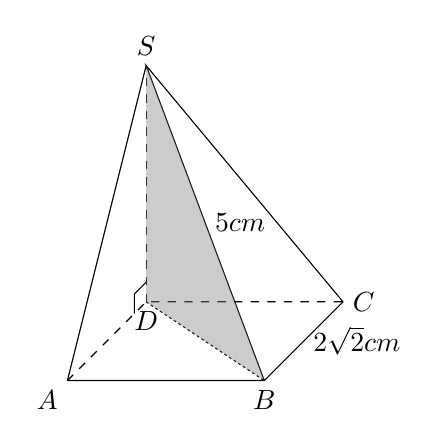
\begin{tikzpicture}
                      \tikzstyle{point}=[circle,thick,draw=black,fill=black,inner sep=0pt,minimum width=4pt,minimum height=4pt]
                      \node (a) at (0,0) {};
                      \node (b) at (2.5,0) {};
                      \node (c) at (3.5,1) {};
                      \node (d) at (1,1) {};
                      \node (e) at (1,4) {};
                      \draw (a.center) node [below left] {$A$} -- (b.center) node [below] {$B$} -- (c.center) node [ right] {$C$} node [midway, right] {$2\sqrt{2}cm$} -- (e.center) node [above] {$S$} -- (b.center) node [midway, right] {$5cm$};
                      \draw (a.center) -- (e.center);
                      \draw[dashed] (a.center) -- (d.center) -- (c.center);
                      \draw[dashed] (d.center) node [below] {$D$} -- (e.center);
                      \draw (1, 1.25) -- (0.85, 1.1) -- (0.85, 0.85);
                      \draw[dash pattern=on 1pt off 1pt] (d.center) -- (b.center);
                      \fill [fill=gray, opacity=0.4] (d.center) -- (b.center) -- (e.center) -- cycle;
                  \end{tikzpicture}
              \end{center}
        \item The diagram below shows a right prism with a rectangular base $ABCD$ with
              length of $28cm$ and width of $20cm$. Assume that plane $VBC$ and the base of
              the pyramid forms a $60^\circ$ angle. Find the angle formed by plane $VAB$ and
              the base.
              \begin{center}
                  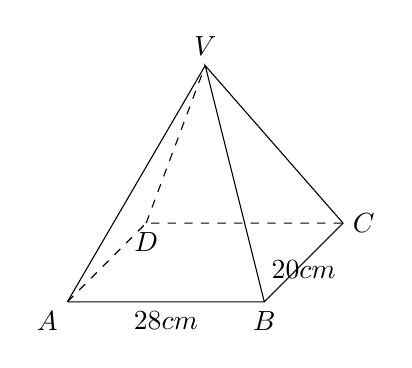
\begin{tikzpicture}
                      \tikzstyle{point}=[circle,thick,draw=black,fill=black,inner sep=0pt,minimum width=4pt,minimum height=4pt]
                      \node (a) at (0,0) {};
                      \node (b) at (2.5,0) {};
                      \node (c) at (3.5,1) {};
                      \node (d) at (1,1) {};
                      \node (e) at (1.75,3) {};
                      \draw (a.center) node [below left] {$A$} -- (b.center) node [below] {$B$} node [midway, below] {$28cm$} -- (c.center) node [ right] {$C$} node [midway, right=12pt, below=-4pt] {$20cm$} -- (e.center) node [above] {$V$} -- (b.center);
                      \draw (a.center) -- (e.center);
                      \draw[dashed] (a.center) -- (d.center) -- (c.center);
                      \draw[dashed] (d.center) node [below] {$D$} -- (e.center);
                  \end{tikzpicture}
              \end{center}
        \item The diagram below shows a regular cuboid with a square base. Given that $VE =
                  \frac{5}{2}AD$. Find:
              \begin{enumerate}
                  \item The angle formed by the angle $VA$ and the base $ABCD$.
                  \item The angle formed by plane $VAD$ and the base.
              \end{enumerate}
              \begin{center}
                  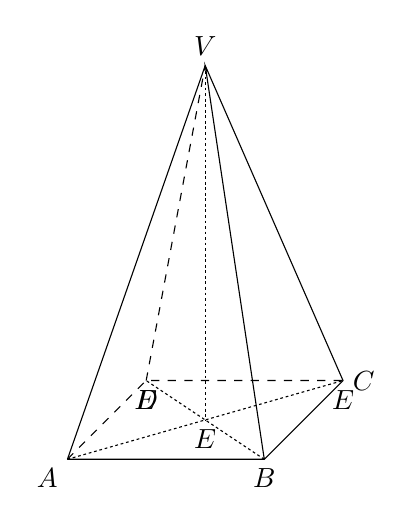
\begin{tikzpicture}
                      \tikzstyle{point}=[circle,thick,draw=black,fill=black,inner sep=0pt,minimum width=4pt,minimum height=4pt]
                      \node (a) at (0,0) {};
                      \node (b) at (2.5,0) {};
                      \node (c) at (3.5,1) {};
                      \node (d) at (1,1) {};
                      \node (e) at (1.75,5) {};
                      \draw (a.center) node [below left] {$A$} -- (b.center) node [below] {$B$} -- (c.center) node [ right] {$C$} -- (e.center) node [above] {$V$} -- (b.center);
                      \draw (a.center) -- (e.center);
                      \draw[dashed] (a.center) -- (d.center) -- (c.center);
                      \draw[dashed] (d.center) node [below] {$D$} -- (e.center);
                      \node (f) at (1.75, 0.5) {};
                      \draw[dash pattern=on 1pt off 1pt] (e.center) -- (f.center) node [below] {$E$};
                      \draw[dash pattern=on 1pt off 1pt] (a.center) -- (c.center) node [below] {$E$};
                      \draw[dash pattern=on 1pt off 1pt] (b.center) -- (d.center) node [below] {$E$};
                  \end{tikzpicture}
              \end{center}
        \item Find the distance from the Panama City$(9^\circ N, 79^\circ 30' W)$ to Toronto
              $(43^\circ 45' N, 79^\circ 30' W)$. (Express your answer in nautical miles)
        \item Tokyo and Adelaide are located at the same longitude, their latitude are
              $35^\circ 45' N$ and $35^\circ S$ respectively. Find the distance between two
              cities along the parallel of latitude.
        \item A plane flies $2000$\emph{NM} along the equator, Find the difference of
              longitude between the point of departure and the destination.
        \item Location $M$ and $N$ are both located at the parallel of latitude $45^\circ$
              north to the equator with a difference in longitude of $20^\circ$. Find the
              distance between $M$ and $N$ along the parallel of latitude. (Express your
              answer in nautical miles)
        \item Location $X$ and $Y$ are on the parallel of latitude $20^\circ$ north to the
              equator, their longitude are $45^\circ E$ and $80^\circ E$ respectively. Find
              the distance between location $X$ and $Y$ along the parallel of latitude.
              (Express your answer in nautical miles)
        \item A plane flies from $A(42^\circ E)$ to $B(20^\circ E)$ along the equator, then
              it flies from $B$ due north to $C(30^\circ N)$. Find the distance the plane
              flies in total.
        \item Assume that $A$ is located $1000$\emph{NM} due north of the equator,
              $600$\emph{NM} due east of the Greenwich Meridian, find the longitude and
              latitude of $A$.
        \item A plane flies from $P(15^\circ N, 30^\circ E)$ $2000$\emph{NM} due south to
              $B$, find the longitude and latitude of $B$. Another plane flies from $P$
              $3000$\emph{NM} due east to $C$, find the longitude and latitude of $C$.
        \item A plane flies from $A(130^\circ E)$ along the equator to $B(120^\circ 30' E)$
              along the equator, then flies from $B$ due north to $C(20^\circ 45')$. Assume
              that the average speed of the plane is $300\text{\emph{NM}}/hr$ throughout the
              journey, find the flight duration for the whole journey.
        \item A plane flies from $A(50^\circ N, 10^\circ E)$ due east to $B(45^\circ E)$.
              \begin{enumerate}
                  \item Find the flight distance of the plane. (Express your answer in nautical miles)
                  \item Assume that the speed of the plane is $420\text{\emph{NM}}/hr$ in average, find
                        the flight duration of the plane.
              \end{enumerate}
        \item Given that three locations $P$, $Q$ and $R$ are located on the same parallel of
              latitude $40^\circ$ north to the equator, The longitude of $P$ and $R$ are
              $10^\circ 30' W$ and $4^\circ 30' E$, $Q$ is located at the middle of $P$ and
              $R$.
              \begin{enumerate}
                  \item Find the difference of longitude between $P$ and $R$.
                  \item Find the longitude of $Q$.
                  \item Find the distance between $P$ and $R$ along the parallel of latitude.
                  \item A ship sails from $P$ to $Q$ along the parallel of latitude with a speed of
                        $18\text{\emph{NM}}/hr$, find the sailing duration of the ship.
              \end{enumerate}
    \end{enumerate}
\end{multicols}
\end{document}